\section{Parameter Tuning}\label{sec:parameter_tuning}

With a few exceptions, all acceptance criteria described in \Cref{sec:acceptance_criteria} depend on one or more parameters.
To tune these parameters an algorithmic approach is preferred to a manual one in order to avoid bias toward acceptance criteria that the authors know well.
A substantial amount of literature is available on algorithms for automatic parameter tuning, and some prominent examples are described in the works by \citet{Birattari2010} and \citet{hutter2009paramils}.
In this work we have implemented a simple iterated local search procedure to perform parameter tuning, as described below.

% We choose to implement our own parameter tuning algorithm instead of using an existing package for transparency reasons: we wanted to be sure to understand the inner workings of  the algorithm. We acknowledge that it would be surprising if the proposed tuning algorithm performs as well as state-of-the-art methods.  However, for our purposes this is not a concern since all acceptance criteria are tuned by the same method, allowing a fair comparison.

Given an acceptance criterion and a problem chosen among the ones we consider in this work (CMST, CVRP, Simple CVRP, and QAP), let $N$ be the number of parameters we are tuning.
Let $n$ be the number of integer parameters and $r$ the number of real-valued parameters.
We assume without loss of generality that the parameters are numbered $\alpha_1, \ldots, \alpha_n, \alpha_{n+1}, \ldots, \alpha_{n+r}$, and that $N = n+r$.
The parameter space will then be $\mathcal{P} = \mathbb{N}^n \times \mathbb{R}^r$.

The aim of the parameter tuning is to explore the parameter space, starting from an initial parameter assignment $\alpha^0 = (a^0_1, \ldots, a^0_N) \in \mathcal{P}$, in a certain number $M \in \mathbb{N}$ of iterations, and return the assignment that gives, \emph{on average}, the best results for the acceptance criterion and problem considered.
Let $I_1, \ldots, I_K$ be the instances used for parameter tuning and let $B_1, \ldots, B_K$ be the best objective function values known from the literature for the instances (these might not be the optimal ones, if the instance is open).
For any given parameter assignment $\alpha$, the algorithm is (re-)run $\lambda \in \mathbb{N}$ times, unchanged, on each instance.
This produces $K$ average results, one for each instance, calculated as
\begin{equation*}
  A_{\alpha,k} = \frac{1}{\lambda} \sum_{i = 1}^\lambda v_{\alpha,i,k}
\end{equation*}
where $v_{\alpha,i,k}$ is the solution value obtained by the algorithm for instance $I_k$ at the $i$-th rerun, with parameter assignment $\alpha$.

We can then calculate the deviation from the best known result, for each instance:
\begin{equation*}
  D_{\alpha,k} = \frac{A_{\alpha,k} - B_k}{A_{\alpha,k}}
\end{equation*}
The score of assignment $\alpha$ is calculated as the average deviation across all instances:
\begin{equation*}
  S_\alpha = \frac{1}{K} \sum_{k = 1}^{K} D_{\alpha,k}
\end{equation*}
The lower the score and, in particular, the closer it is to 0, the better is the parameter assignment $\alpha$.

\begin{algorithm}[ht]
  \caption{Parameter Tuning Algorithm}\label{alg:par_tuning}
  \SetKwInOut{Input}{Input}

  \Input{Initial parameters $\alpha^0$}
  \Input{Initial steps: $\sigma^0$}

  \For{$k = 1, \ldots, M$}{
    $\alpha^\textup{new} = \textup{BestInNb}(\alpha^{k-1}, \sigma^{k-1})$\;\nllabel{ln:explore_nb}

    \eIf{$\alpha^\textup{new} \neq \alpha^{k-1}$}{
      $\alpha^k = \alpha^\textup{new}$\;
      $\sigma^k = \sigma^{k-1}$\;
    }{
      $\alpha',\alpha'' = \textup{BestTwo}()$\;\nllabel{ln:best_two}
      $\alpha^k = \textup{NewCentre}(\alpha', \alpha'')$\;\nllabel{ln:new_centre}
      $\sigma^k = \textup{NewSteps}(\alpha', \alpha'')$\;\nllabel{ln:new_steps}

      \If{$\alpha^k = \alpha^\textup{new} \textup{ or StepsTooSmall}(\sigma^k)$}{\nllabel{ln:diversify_condition}
        $\alpha^k = \textup{Diversify}(\alpha^k)$\;\nllabel{ln:diversify}
        $\sigma^k = \sigma^0$\;\nllabel{ln:reset_steps}
      }
    }
  }

  \Return{$\argmin_{k = 1, \ldots, M} \left\{ S_{\alpha^k} \right\}$}
\end{algorithm}

A general overview of the parameter tuning algorithm is given in \Cref{alg:par_tuning}.
An initial parameter assignment $\alpha^0$ is given, together with an initial step $\sigma^0$.
The step defines the neighbourhood of the current assignment:
\begin{equation}
  \mathcal{N}(\alpha) = \left\{ ( \alpha'_1, \ldots, \alpha'_N ) \; | \; \alpha'_i - \alpha_i \in \{ -\sigma_i, 0, \sigma_i \} \; \forall i = 1, \ldots, N \right\}
\end{equation}
The neighbourhood is defined by all possible combination of moves, in all the directions defined by the components of the parameter vector, each by its corresponding step, with $\sigma^0_1, \ldots, \sigma^0_n \in \mathbb{N}$ and $\sigma^0_{n+1}, \ldots, \sigma^0_N \in \mathbb{R}$.
For larger values of $N$, the exploration of the neighbourhood defined above is computationally expensive.
Therefore, for values of $N \geq 3$, we define the alternative neighbourhood:
\begin{align}
  \mathcal{N}(\alpha) = \{ & (\alpha'_1, \ldots, \alpha'_N) \; | \nonumber \\
  &\exists i \in \{ 1, \ldots, N \} \, : \, \alpha'_i - \alpha_i \in \{ -\sigma_i, 0, \sigma_i \} \text{ and } \nonumber \\
  &\forall j \neq i \;\; \alpha'_j = \alpha_j \} \label{eq:smallN}
\end{align}
According to definition \eqref{eq:smallN}, therefore, we can only move along one direction at a time.
\Cref{fig:N2} and \Cref{fig:N3} give a graphical representation of $\mathcal{N}(\alpha)$ for $N = 2$ and $N = 3$.

\begin{figure}\centering
    \begin{subfigure}[t]{0.45\textwidth}\centering
        \resizebox{\textwidth}{!}{%
        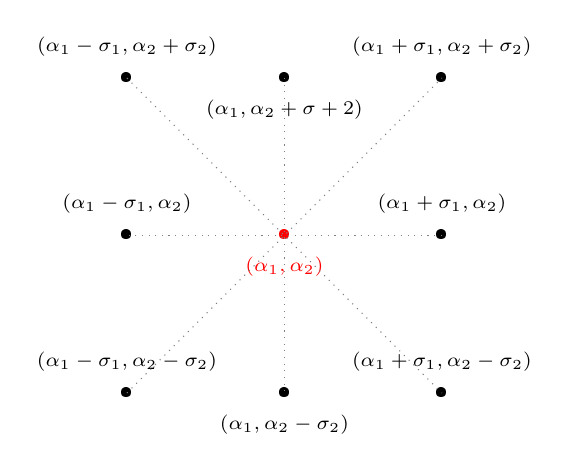
\begin{tikzpicture}
          \node at (-2,-1.6) {\scriptsize$(\alpha_1 - \sigma_1, \alpha_2 - \sigma_2)$};
          \node at (-2,-2) {\textbullet};

          \node at (-2,0.4) {\scriptsize$(\alpha_1 - \sigma_1, \alpha_2)$};
          \node at (-2,0) {\textbullet};

          \node at (-2,2.4) {\scriptsize$(\alpha_1 - \sigma_1, \alpha_2 + \sigma_2)$};
          \node at (-2,2) {\textbullet};

          \node at (0,-2.4) {\scriptsize$(\alpha_1, \alpha_2 - \sigma_2)$};
          \node at (0,-2) {\textbullet};

          \node[red] at (0,-0.4) {\scriptsize$(\alpha_1, \alpha_2)$};
          \node[red] at (0,0) {\textbullet};

          \node at (0,1.6) {\scriptsize$(\alpha_1, \alpha_2 + \sigma+2)$};
          \node at (0,2) {\textbullet};

          \node at (2,-1.6) {\scriptsize$(\alpha_1 + \sigma_1, \alpha_2 - \sigma_2)$};
          \node at (2,-2) {\textbullet};

          \node at (2,0.4) {\scriptsize$(\alpha_1 + \sigma_1, \alpha_2)$};
          \node at (2,0) {\textbullet};

          \node at (2,2.4) {\scriptsize$(\alpha_1 + \sigma_1, \alpha_2 + \sigma_2)$};
          \node at (2,2) {\textbullet};

          \draw[dotted,black!50] (-2,-2) -- (0,0) -- (2,2);
          \draw[dotted,black!50] (-2,2) -- (0,0) -- (2,-2);
          \draw[dotted,black!50] (0,2) -- (0,0) -- (0,-2);
          \draw[dotted,black!50] (2,0) -- (0,0) -- (-2,0);
        \end{tikzpicture}}
        \caption{\footnotesize Case $N = 2$.}\label{fig:N2}
    \end{subfigure}
    \hfill
    \begin{subfigure}[t]{0.45\textwidth}\centering
        \resizebox{\textwidth}{!}{%
        \begin{tikzpicture}
          \node[red] at (0,0.4) {\scriptsize$(\alpha_1,\alpha_2,\alpha_3)$};
          \node[red] at (0,0) {\textbullet};

          \node at (2,-0.4) {\scriptsize$(\alpha_1+\sigma_1,\alpha_2,\alpha_3)$};
          \node at (2,0) {\textbullet};

          \node at (-2,-0.4) {\scriptsize$(\alpha_1-\sigma_1,\alpha_2,\alpha_3)$};
          \node at (-2,0) {\textbullet};

          \node at (0,2.4) {\scriptsize$(\alpha_1,\alpha_2+\sigma_2,\alpha_3)$};
          \node at (0,2) {\textbullet};

          \node at (0,-2.4) {\scriptsize$(\alpha_1,\alpha_2-\sigma_2,\alpha_3)$};
          \node at (0,-2) {\textbullet};

          \node at (-2.2,-1.7) {\scriptsize$(\alpha_1,\alpha_2,\alpha_3-\sigma_3)$};
          \node at (-1.414,-1.414) {\textbullet};

          \node at (2.2,1.7) {\scriptsize$(\alpha_1,\alpha_2,\alpha_3+\sigma_3)$};
          \node at (1.414,1.414) {\textbullet};

          \draw[dotted,black!50] (-2,0) -- (0,0) -- (2,0);
          \draw[dotted,black!50] (0,2) -- (0,0) -- (0,-2);
          \draw[dotted,black!50] (-1.414,-1.414) -- (0,0) -- (1.414,1.414);
        \end{tikzpicture}}
        \caption{\footnotesize Case $N = 3$. The diagonal dotted lines represent movement along a third axis.}\label{fig:N3}
    \end{subfigure}
    \caption{Representation of neighbourhood $\mathcal{N}(\alpha)$.}
\end{figure}

At each iteration of the algorithm, the next parameter assignment is chosen in the neighbourhood of the current one (line \ref{ln:explore_nb}) as the one with the best score:
\begin{equation*}
  \alpha^{k+1} = \argmin \left\{ S_{\alpha'} \ | \ \alpha' \in \mathcal{N}(\alpha^k) \right\}
\end{equation*}
When $\alpha^{k+1} = \alpha^k$, we have reached a local optimum and the search must be interrupted and restarted somewhere else in the parameter space. In order to do this, we retrieve the best and second-best parameter configuration encoutered during the whole search, $\alpha'$ and $\alpha''$ respectively (line \ref{ln:best_two}), and we set the current parameter configuration as the centre of mass between $\alpha'$ and $\alpha''$ (line \ref{ln:new_centre}):
\begin{equation*}
  \alpha^k = \left( \frac{\alpha'_1 + \alpha''_1}{2}, \ldots, \frac{\alpha'_N + \alpha''_N}{2} \right)
\end{equation*}
where integer components are rounded to the nearest integer. The step sizes are also recalculated (line \ref{ln:new_steps}) and set as:
\begin{equation*}
  \sigma^k = \left( \frac{|\alpha'_1 - \alpha''_1|}{3}, \ldots, \frac{|\alpha'_N - \alpha''_N|}{3} \right)
\end{equation*}
and, again, integer components are rounded. If, after recalculating $\alpha^k$, all steps are below their minimum step size (which is a predetermined parameter), or if it happened that $\alpha^k$ did not change (line \ref{ln:diversify_condition}) we proceed with a stronger diversification (line \ref{ln:diversify}) and we reset the step sizes (line \ref{ln:reset_steps}). The strong diversification consists in setting:
\begin{equation*}
  \alpha^k = \left( \alpha^{k-1}_1 + \rho_1 \sigma^0_1, \ldots, \alpha^{k-1}_N + \rho_N \sigma^0_N \right)
\end{equation*}
where each $\rho_i$ is taken randomly from the intervals $[-3,-1]\cup[1,3]$.

\Cref{tbl:par_tuning_summary1,tbl:par_tuning_summary2} summarise the results of parameter tuning for the problems considered, using six tuning instances for each problem.
Column ``Acceptance Criterion'' shows the acceptance criteria, column ``Score'' gives the value of $S_{\alpha^*}$ for the best parameter assignment $\alpha^* \in \mathcal{P}$, while column ``Parameters'' gives the values of the parameters in $\alpha^*$, using the same notation as in \Cref{sec:acceptance_criteria}.
The maximum number of tuning iterations has been set to $M = 20$, the number of reruns to $\lambda = 10$ and the number of iterations of each run (exit criterion) to 150,000.

\begin{sidewaystable}\centering\scriptsize
    \begin{tabular}{l lL{5cm} lL{5cm}}
        \toprule
        & \multicolumn{2}{c}{\textbf{CMST}} & \multicolumn{2}{c}{\textbf{CVRP}} \\
        \midrule\rule{0pt}{3ex}%
        Acceptance Criterion & Score & Parameters & Score & Parameters \\
        \cmidrule(r){1-1}\cmidrule(lr){2-3}\cmidrule(lr){4-5}
        GD                       & $2.216 \cdot 10^{-2}$ & $\alpha = 1.0167, \beta = 0.0001$ & $1.386 \cdot 10^{-2}$ & $\alpha = 1.0167, \beta = 0.0002$ \\
        HC                       & $4.563 \cdot 10^{-2}$ & & $1.890 \cdot 10^{-2}$ & \\
        LAHC                     & $1.960 \cdot 10^{-2}$ & $L = 22500$ & $1.397 \cdot 10^{-2}$ & $L = 15000$ \\
        Improved LAHC            & $2.024 \cdot 10^{-2}$ & $L = 9180$ & $1.340 \cdot 10^{-2}$ & $L = 4166$ \\
        NLGD                     & $2.794 \cdot 10^{-2}$ & $\alpha = 2.1714, \beta = 0.0465, \gamma = 0.1057, \delta = 0.0096$ & $1.470 \cdot 10^{-2}$ & $\alpha = 1.2500, \beta = 0.0075, \gamma = 0.0208, \delta = 0.0100$ \\
        RW                       & $5.828 \cdot 10^{-2}$ & & $3.062 \cdot 10^{-2}$ & \\
        Lin. RRT                 & $1.776 \cdot 10^{-2}$ & $T^\textup{start} = 0.0750, T^\textup{end} = 0.0037$ & $9.060 \cdot 10^{-3}$ & $T^\textup{start} = 0.0222, T^\textup{end} = 0.0000$ \\
        Lin. RRT (fixed end)     & $1.773 \cdot 10^{-2}$ & $T^\textup{start} = 0.0500$ & $8.733 \cdot 10^{-3}$ & $T^\textup{start} = 0.0167$ \\
        Exp. RRT                 & $2.044 \cdot 10^{-2}$ & $T^\textup{start} = 0.0250, T^\textup{end} = 0.0289$ & $1.133 \cdot 10^{-2}$ & $T^\textup{start} = 0.0042, T^\textup{end} = 0.0376$ \\
        Exp. SA with Ad. Probab. & $1.649 \cdot 10^{-2}$ & $h^\textup{start} = 9.7500, h^\textup{end} = 2.0093$ & $1.218 \cdot 10^{-2}$ & $h^\textup{start} = 4.7500, h^\textup{end} = 0.6944$ \\
        Exp. SA                  & $1.698 \cdot 10^{-2}$ & $h^\textup{start} = 0.1128, h^\textup{end} = 0.0104$ & $1.130 \cdot 10^{-2}$ & $h^\textup{start} = 0.1211, h^\textup{end} = 0.0004$ \\
        Lin. SA                  & $1.606 \cdot 10^{-2}$ & $h^\textup{start} = 11.500, h^\textup{end} = 1.7917$ & $1.132 \cdot 10^{-2}$ & $h^\textup{start} = 3.7500, h^\textup{end} = 0.4097$ \\
        Lin. SA (fixed end)      & $1.651 \cdot 10^{-2}$ & $h^\textup{start} = 12.193$ & $1.180 \cdot 10^{-2}$ & $h^\textup{start} = 6.8152$ \\
        Instance-scaled Exp. SA  & $1.601 \cdot 10^{-2}$ & $h^\textup{start} = 13.507, h^\textup{end} = 2.0903, M = 1.0000$ & $1.122 \cdot 10^{-2}$ & $h^\textup{start} = 4.2083, h^\textup{end} = 0.6181, M = 1.0000$ \\
        Exp. SA with Reheating   & $1.611 \cdot 10^{-2}$ & $h^\textup{start} = 12.000, h^\textup{end} = 1.8750, r = 3.5000, R = 1.0000$ & $1.138 \cdot 10^{-2}$ & $h^\textup{start} = 13.500, h^\textup{end} = 0.6250, r = 0.5000, R = 1.0000$ \\
        Lin. TA                  & $1.648 \cdot 10^{-2}$ & $T^\textup{start} = 0.0708, T^\textup{end} = 0.0014$ & $1.099 \cdot 10^{-2}$ & $T^\textup{start} = 0.0250, T^\textup{end} = 0.0000$ \\
        Lin. TA (fixed end)      & $1.667 \cdot 10^{-2}$ & $T^\textup{start} = 0.0875$ & $1.123 \cdot 10^{-2}$ & $T^\textup{start} = 0.0292$ \\
        Exp. TA                  & $2.259 \cdot 10^{-2}$ & $T^\textup{start} = 0.0125, T^\textup{end} = 0.0023$ & $1.296 \cdot 10^{-2}$ & $T^\textup{start} = 0.0016, T^\textup{end} = 0.0017$ \\
        Exp. WA                  & $1.794 \cdot 10^{-2}$ & $p^\textup{start} = 0.7851, p^\textup{end} = 0.0979$ & $1.754 \cdot 10^{-2}$ & $p^\textup{start} = 0.0500, p^\textup{end} = 0.0150$ \\
        Lin. WA                  & $1.819 \cdot 10^{-2}$ & $p^\textup{start} = 0.6580, p^\textup{end} = 0.0430$ & $1.744 \cdot 10^{-2}$ & $p^\textup{start} = 0.1500, p^\textup{end} = 0.0167$ \\
        Lin. WA (fixed end)      & $1.867 \cdot 10^{-2}$ & $p^\textup{start} = 0.5500$ & $1.426 \cdot 10^{-2}$ & $p^\textup{start} = 1.0000$ \\
        \bottomrule
    \end{tabular}
    \caption{Parameter tuning results sumamry for CMST and CVRP.}\label{tbl:par_tuning_summary1}
\end{sidewaystable}

\begin{sidewaystable}\centering\scriptsize
    \begin{tabular}{l lL{4cm} lL{5cm} lL{5cm}}
        \toprule
        & \multicolumn{2}{c}{\textbf{Simple LNS for CVRP}} & \multicolumn{2}{c}{\textbf{QAP}} \\
        \midrule\rule{0pt}{3ex}%
        Acceptance Criterion & Score & Parameters & Score & Parameters \\
        \cmidrule(r){1-1}\cmidrule(lr){2-3}\cmidrule(lr){4-5}
        GD                       & $3.362 \cdot 10^{-2}$ & $\alpha = 1.1241, \beta = 0.0002$                                            & $1.167 \cdot 10^{-2}$ & $\alpha = 1.0117, \beta = 0.0001$                                            \\
        HC                       & $4.845 \cdot 10^{-2}$ &                                                                              & $2.909 \cdot 10^{-2}$ &                                                                              \\
        LAHC                     & $3.516 \cdot 10^{-2}$ & $L = 10833$                                                                  & $1.974 \cdot 10^{-2}$ & $L = 17500$                                                                  \\
        Improved LAHC            & $3.472 \cdot 10^{-2}$ & $L = 4248$                                                                   & $1.677 \cdot 10^{-2}$ & $L = 7431$                                                                   \\
        NLGD                     & $3.481 \cdot 10^{-2}$ & $\alpha = 1.1042, \beta = 0.0050, \gamma = 0.0000, \delta = 0.0183$          & $2.124 \cdot 10^{-2}$ & $\alpha = 1.7500, \beta = 0.0150, \gamma = 0.0167, \delta = 0.0125$          \\
        RW                       & $4.730 \cdot 10^{-2}$ &                                                                              & $3.072 \cdot 10^{-2}$ &                                                                              \\
        Lin. RRT                 & $2.333 \cdot 10^{-2}$ & $T^\textup{start} = 0.0176, T^\textup{end} = 0.0000$                         & $0.996 \cdot 10^{-2}$ & $T^\textup{start} = 0.1664, T^\textup{end} = 0.0002$                         \\
        Lin. RRT (fixed end)     & $2.405 \cdot 10^{-2}$ & $T^\textup{start} = 0.0222$                                                  & $1.019 \cdot 10^{-2}$ & $T^\textup{start} = 0.2558$                                                  \\
        Exp. RRT                 & $2.679 \cdot 10^{-2}$ & $T^\textup{start} = 0.0125, T^\textup{end} = 0.0906$                         & $1.421 \cdot 10^{-2}$ & $T^\textup{start} = 0.1000, T^\textup{end} = 0.0250$                         \\
        Exp. SA with Ad. Probab. & $2.862 \cdot 10^{-2}$ & $h^\textup{start} = 20.273, h^\textup{end} = 0.5141$                         & $1.340 \cdot 10^{-2}$ & $h^\textup{start} = 9.7500, h^\textup{end} = 1.2083$                         \\
        Exp. SA                  & $2.647 \cdot 10^{-2}$ & $h^\textup{start} = 0.1367, h^\textup{end} = 0.0008$                         & $1.286 \cdot 10^{-2}$ & $h^\textup{start} = 7.6359, h^\textup{end} = 0.0002$                         \\
        Lin. SA                  & $2.788 \cdot 10^{-2}$ & $h^\textup{start} = 9.0000, h^\textup{end} = 0.0000$                         & $1.309 \cdot 10^{-2}$ & $h^\textup{start} = 9.5000, h^\textup{end} = 1.5833$                         \\
        Lin. SA (fixed end)      & $2.750 \cdot 10^{-2}$ & $h^\textup{start} = 12.347$                                                  & $1.132 \cdot 10^{-2}$ & $h^\textup{start} = 12.000$                                                  \\
        Instance-scaled Exp. SA  & $2.733 \cdot 10^{-2}$ & $h^\textup{start} = 14.229, h^\textup{end} = 0.6250, M = 1.0000$             & $1.411 \cdot 10^{-2}$ & $h^\textup{start} = 12.000, h^\textup{end} = 2.0000, M = 1.0000$             \\
        Exp. SA with Reheating   & $2.821 \cdot 10^{-2}$ & $h^\textup{start} = 12.750, h^\textup{end} = 0.7500, r = 2.4167, R = 2.5833$ & $1.347 \cdot 10^{-2}$ & $h^\textup{start} = 12.250, h^\textup{end} = 1.7292, r = 3.2500, R = 2.8750$ \\
        Lin. TA                  & $2.599 \cdot 10^{-2}$ & $T^\textup{start} = 0.0212, T^\textup{end} = 0.0003$                         & $1.847 \cdot 10^{-2}$ & $T^\textup{start} = 0.0500, T^\textup{end} = 0.0000$                         \\
        Lin. TA (fixed end)      & $2.597 \cdot 10^{-2}$ & $T^\textup{start} = 0.0208$                                                  & $1.800 \cdot 10^{-2}$ & $T^\textup{start} = 0.0419$                                                  \\
        Exp. TA                  & $3.087 \cdot 10^{-2}$ & $T^\textup{start} = 0.0033, T^\textup{end} = 0.0059$                         & $1.613 \cdot 10^{-2}$ & $T^\textup{start} = 0.0500, T^\textup{end} = 0.0013$                         \\
        Exp. WA                  & $3.121 \cdot 10^{-2}$ & $p^\textup{start} = 1.0000, p^\textup{end} = 0.1090$                         & $1.002 \cdot 10^{-2}$ & $p^\textup{start} = 0.4500, p^\textup{end} = 0.0517$                         \\
        Lin. WA                  & $2.974 \cdot 10^{-2}$ & $p^\textup{start} = 1.0000, p^\textup{end} = 0.0022$                         & $0.932 \cdot 10^{-2}$ & $p^\textup{start} = 0.3000, p^\textup{end} = 0.0300$                         \\
        Lin. WA (fixed end)      & $3.046 \cdot 10^{-2}$ & $p^\textup{start} = 0.9833$                                                  & $1.029 \cdot 10^{-2}$ & $p^\textup{start} = 0.3833$                                                  \\
        \bottomrule
    \end{tabular}
    \caption{Parameter tuning results sumamry for Simple CVRP and QAP.}\label{tbl:par_tuning_summary2}
\end{sidewaystable}